\chapter{Evaluation}
\label{chap:evaluation}

Dieses Kapitel widmet sich der Auswertung der Ergebnisse anhand verschiedener Metriken. Eingebettet in der Transformationssoftware befindet sich ein Präprozessor, der die aufgenommen Daten vor der Transformation manipulieren kann. Auf diese Weise werden mehrere Trainingsdatensätze erstellt, die in der Evaluation daraufhin analysiert werden, wie genau ein Klassifikator nach dem Training mit ihnen Vorhersagen treffen kann.

Die folgenden Datensätze werden generiert:

\begin{enumerate}
\item \textit{Combined}: Alle Daten werden ohne Veränderungen mit in die Transformation einbezogen.
\item \textit{NoisyBandTimestamps}: Die Zeitstempel der Readings des Bands werden mit gaussschem Rauschen versehen
\item \textit{Band combined}: Alle Daten des Smartphones werden vor der Transformation verworfen, sodass nur noch die Daten des Band verbleiben..
\item \textit{Band accel}: Nur die Daten des Beschleunigungssensors des Microsoft Band 2 werden mit in die Transformation einbezogen.
\item \textit{Band gyro}: Nur die Daten des Gyroskops des Microsoft Band 2 werden mit in die Transformation einbezogen.
\item \textit{Phone comb.}: Alle Daten des Microsoft Band 2 werden vor der Transformation verworfen, sodass nur noch die Daten des Smartphones verbleiben.
\item \textit{Phone accel}: Nur die Daten des Beschleunigungssensors des Smartphones werden mit in die Transformation einbezogen.
\item \textit{Phone gyro}: Nur die Daten des Gyroskops des Smartphones werden mit in die Transformation einbezogen.
\item \textit{SamplingRate1Hz}: Es werden Readings verworfen, als hätten Band und Smartphone jeweils nur Readings bei einer Rate von 1 Hz geliefert.
\item \textit{SamplingRate5Hz}: Es werden Readings verworfen, als hätten Band und Smartphone jeweils nur Readings bei einer Rate von 5 Hz geliefert.
\end{enumerate}

\todo{Genauigkeiten aus Weiss zum Vergleich mit einbinden, side by side in einem diagramm}

\section{Effektivität der Datenkombination}
In diesem Abschnitt widmen wir uns der Frage, wie effektiv die Kombination der Daten von Band und Smartphone hinsichtlich der Vorhersagegenauigkeit gegenüber einer einzigen Datenquelle ist. Weiss et al.\cite{Weiss2016} werten in ihrem Papier die Genauigkeit von Modellen aus, die entweder auf Daten des Beschleunigungssensors eines Smartphones, des Beschleunigungssensors einer Smartwatch oder des Gyroskops einer Smartwatch zurückgreifen. Eine Kombination der Daten schlagen die Autoren vor, führen diese allerdings nicht durch.

Tabelle~\ref{tab:accuracy-personal} zeigt die Genauigkeit der persönlichen Modelle und Tabelle~\ref{tab:accuracy-impersonal} die der unpersönlichen Modelle. Ein persönliches Modell basiert auf Daten des jeweiligen Benutzers, während ein unpersönliches Modell noch keine Daten des Nutzers gesehen hat, für den eine Vorhersage getroffen werden soll. Die \textit{Genauigkeit} ist definiert als der Anteil der korrekt klassifizierten Instanzen, die dem Modell zum Test vorgelegt wurden.

Die erste Spalte der in diesem Abschnitt referenzierten Tabellen gibt den Algorithmus an, der zur Klassifikation verwendet wurde. Eine Erläuterung der Algorithmen ist in Abschnitt~\ref{section:ml-algos}
zu finden. Fettgedruckt ist immer der jeweils höchste Wert einer Spalte.

\subsection{Persönliche Modelle}

Die Evaluierung der persönlichen Modelle erfolgt wie folgt: Für jeden Benutzer $b$ wird eine 10-fache Kreuzvalidierung durchgeführt, wobei die Trainingsdaten nur Daten von $b$ beinhalten. Anschließend wird der Durchschnitt der einzelnen Genauigkeiten über alle Benutzer gebildet, um einen globalen Genauigkeitswert zu erhalten.

Nutzt man nur je ein Gyroskop, ist die Qualität der persönlichen Modelle am schlechtesten. Im Gegensatz dazu haben bereits Modelle, die lediglich Daten von einem der Beschleunigungssensoren verwenden, eine gute Aussagekraft. Weiss et al.\cite{Weiss2016} stellten in ihrem Experiment fest, dass die Genauigkeit des \textit{Phone accel}-Modells $17.8 \%$ über dem \textit{Watch accel / Band accel}-Modell lag. In unserem Experiment ist der Unterschied trotz gleichem Experimentaufbau mit $1.6 \%$ weit geringer. Eine denkbare Erklärung wäre, dass die Probanden von Weiss et al. über verschiedene Aktivitäten hinweg mehr Variation bei ihrer Bewegung des Unterkörpers eingebracht haben könnten.

Vergleicht man die beste Datenquelle (Band accel) mit den Kombinationsmöglichkeiten, so lässt sich feststellen, dass die Hinzunahme der anderen Sensoren des Band eine Genauigkeit von $97.1 \%$ erzielt, wohingegen die Kombination der beiden Smartphone-Sensoren lediglich eine Verbesserung von $0.7 \%$ gegenüber \textit{Phone accel} und gegenüber \textit{Band accel} sogar eine Verschlechterung erwirkt. Hebt man jedoch die künstlichen Einschränkungen auf, so wird eine Genauigkeit von $99.4 \%$ erreicht, sodass Benutzer nach dreiminütiger Aufnahme einer Aktivität davon ausgehen könnten, dass diese in Zukunft in aller Regel automatisch erkannt wird. Insgesamt konnte gegenüber \textit{Phone Accel} damit eine Verbesserung um $7.8 \%$ erreicht werden, obwohl die Verbesserung einer bereits hohen Genauigkeit herausfordernd ist.\todo{Kann man das belegen?} Gegenüber dem besten Ergebnis eines einzelnen Sensors (\textit{Band accel}) mit $75.2 \%$ liefert die Kombination aller Daten eine Verbesserung um $7.8 \%$.

\subsection{Unpersönliche Modelle}
Für die Evaluierung der unpersönlichen Modelle wird eine Kreuzvalidierung über die Nutzer durchgeführt, das heißt der Datensatz $D$ wird für alle Benutzer $b$ aufgeteilt in $D = \text{Train} \uplus \text{Test}$ mit $\text{Train} = \{\text{Intervall ist nicht von } b\}, \text{Test} = D \backslash \text{Train}$.

Das schlechteste Ergebnis wird mit $35.1 \%$ bei den unpersönlichen Modellen erzielt, wenn nur das Gyroskop des Smartphones verwendet wird. Nur wenig besser sind die Modelle, die nur den Beschleunigungssensor des Smartphones ($39.2 \%$) oder beide Sensoren des Smartphones ($41.3 \%$) nutzen. Für den praktischen Gebrauch sind diese Modelle aufgrund ihrer Ungenauigkeit untauglich. Schon rund $20 \%$ besser sind die Modelle, die nur das Gyroskop des Bands nutzen, wobei der Wechsel zum Beschleunigungssensor eine weitere Verbesserung um fast $14 \%$ ermöglicht. Offenbar erklären die Daten des Beschleunigungssensors einen Großteil der Daten, die auch durch das Gyroskop und die anderen Sensoren des Band erklärt werden, sodass eine Kombination aller Band-Sensoren lediglich ein Verbesserung um rund $1 \%$ ermöglicht. Selbiges gilt auch für die Hinzunahme der Daten des Smartphones: Es wird eine Verbesserung um $2 \%$ erzielt, was darauf schließen lässt, dass die Armbewegungen unter den Probanden ähnlich sind, die Bewegungen auf Hüfthöhe hingegen weniger. Gegenüber dem besten Ergebnis eines einzelnen Sensors (\textit{Band accel}) mit $75.2 \%$ liefert die Kombination aller Daten eine Verbesserung um $3.3 \%$.

\begin{table}
\centering
\begin{tabular}{|c|c|c|c|c|c|c|c|}
	\hline 
	\textbf{Algo.} & \textbf{Phone accel} & \textbf{Phone gyro} & \textbf{Band accel} & \textbf{Band gyro} & \textbf{Comb.} & \textbf{Band comb.} & \textbf{Phone comb.} \\ 
	\hline 
	RF & 88.7 & \textbf{68.2} & \textbf{91.6} & \textbf{80.5} & \textbf{99.4} & \textbf{97.1} & \textbf{90.7} \\ 
	J48 & \textbf{90.0} & 64.3 & 86.5 & 72.7 & 92.8 & 90.1 & 89.7 \\ 
	IB3 & 62.2 & 44.8 & 77.0 & 59.4 & 82.3 & 76.9 & 60.1 \\ 
	NB & 87.6 & 60.4 & 90.9 & 78.8 & 96.2 & 92.2 & 85.5 \\ 
	MLP & 78.9 & 51.5 & 88.9 & 67.8 & 94.8 & 90.7 & 75.1 \\ 
	\hline 
	$\varnothing$ & 81.5 & 57.8 & 87.0 & 71.8 & 93.1 & 89.4 & 80.2 \\ 
	\hline 
\end{tabular}
\caption{Genauigkeit der persönlichen Modelle in Prozent}
\label{tab:accuracy-personal}
\end{table}

\begin{table}
\centering
\begin{tabular}{|c|c|c|c|c|c|c|c|}
	\hline 
	\textbf{Algo.} & \textbf{Phone accel} & \textbf{Phone gyro} & \textbf{Band accel} & \textbf{Band gyro} & \textbf{Comb.} & \textbf{Band comb.} & \textbf{Phone comb.} \\ 
	\hline 
	RF & \textbf{39.2} & \textbf{35.1} & \textbf{75.2} & \textbf{61.7} & \textbf{78.5} & \textbf{76.5} & \textbf{41.3} \\ 
	J48 & 32.9 & 29.1 & 61.6 & 49.2 & 59.7 & 61.3 & 32.6 \\ 
	IB3 & 24.3 & 22.6 & 60.9 & 45.0 & 52.9 & 58.0 & 26.0 \\ 
	NB & 31.8 & 30.0 & 67.3 & 56.9 & 60.9 & 62.3 & 35.0 \\ 
	MLP & 28.8 & 29.3 & 70.3 & 53.5 & 54.9 & 74.3 & 31.5 \\ 
	\hline 
	$\varnothing$ & 81.5 & 29.2 & 67.1 & 53.3 & 61.4 & 66.5 & 33.3 \\ 
	\hline 
\end{tabular} 
\caption{Genauigkeit der unpersönlichen Modelle in Prozent}
\label{tab:accuracy-impersonal}
\end{table}

\section{Genauigkeit bei ungenauen Zeitstempeln}
Die Problemstellung, Daten mehrerer Quellen miteinander zu kombinieren, wirft die Frage auf, inwiefern die Synchronisierung der Daten einen Einfluss auf die Genauigkeit der resultierenden Modelle besitzt. Smartphone und Band besitzen je eine eigene Uhr, sodass die Datenquellen zum selben Zeitpunkt $t$ \textit{Readings} mit Zeitstempeln $t + \epsilon_\text{Smartphone}$, bzw. $t + \epsilon_\text{Band}$ mit $|\epsilon_\text{Smartphone} - \epsilon_\text{Band}| > 0$ liefern könnten. Wird die Differenz zu groß, schadet die Kombination der Quellen möglicherweise mehr als sie nützt.

Ein erster Ansatz, um dieses Problem zu bekämpfen, war daher zunächst, die beiden Uhren via Bluetooth und ein Verfahren wie das \textit{Network Time Protocol (NTP)} \cite{Mills} zu synchronisieren. Leider ermöglicht das Microsoft Band SDK nicht die Ausführung beliebigen Codes auf dem Band, sondern nur das Abonnieren von Events, die Sensordaten ausliefern. Das SDK versieht diese Events lokal auf dem Smartphone mit Zeitstempeln, sodass weder direkt noch indirekt Zugriff auf die Uhr des Band besteht und eine Synchronisierung somit unmöglich ist.

Um zu prüfen, inwiefern unsere Modelle durch eine mögliche, nicht detektierbare Differenz der Uhren beeinträchtigt werden, generiert die Transformationssoftware zusätzlich zum normalen vollständigen Datensatz auch einen, in dem die Zeitstempel des Bands additiv mit gausschem Rauschen versehen wurden. Die Parameter des gausschen Rauschens wurden auf einen Mittelwert von $0$ und eine Standardabweichung von $500 \text{ms}$ festgelegt. Die Ergebnisse der Auswertung werden in Tabelle~\ref{tab:accuracy-noisy_timestamps} aufgeführt. Betrachtet man die jeweils besten Modelle, so lässt sich sowohl bei den persönlichen, als auch bei den unpersönlichen Modellen eine Verschlechterung um lediglich $0.2 \%$ feststellen. Auch die anderen Modelle sind im Durchschnitt mit Verschlechterungen um $0.3 \%$, bzw. $0.5 \%$ hinreichend resistent gegen das Rauschen.

Um zu prüfen, ob eine Standardabweichung von $500 \text{ms}$ sinnvoll ist, wurde über drei Tage hinweg um jeweils 10, 15 und 18 Uhr geprüft, mit welchem zeitlichen Abstand das Umspringen von der vollen Stunde auf die nächste Minute erfolgte. Eine Verzögerung war in keinem der Fälle mit dem Auge beobachtbar, weshalb davon auszugehen ist, dass die Uhren aufgrund der bereits bestehenden Synchronisierung durch die vom Hersteller gelieferte Band-App für Android in der Regel weniger als $500 \text{ms}$ voneinander abweichen. Dies führt zu der Annahme, dass die Genauigkeit der Zeitstempel im Rahmen dieser Arbeit keinen negativen Einfluss auf die Ergebnisse hat und somit nicht weiter betrachtet werden muss.

\begin{table}
\centering
\begin{tabular}{|c|c|c||c|c|}
	\hline 
	\textbf{Algo.} & \textbf{Comb. (Pers.)} & \textbf{Verrauscht (Pers.)} &\textbf{Comb. (Unpers.)} & \textbf{Verrauscht (Unpers.)} \\ 
	\hline 
	RF & \textbf{99.4} & \textbf{99.2} & \textbf{78.5} & \textbf{78.3} \\ 
	J48 & 92.8 & 93.5 & 59.7 & 57.3 \\ 
	IB3 & 82.3 & 81.5 & 52.9 & 52.9 \\ 
	NB & 96.2 & 95.7 & 60.9 & 60.5 \\ 
	MLP & 94.8 & 94.2 & 54.9 & 55.4 \\ 
	\hline 
	$\varnothing$ & 93.1 & 92.8 & 61.4 & 60.9 \\ 
	\hline
\end{tabular} 
\caption{Genauigkeit der Modelle mit verrauschten Band-Zeitstempeln in Prozent}
\label{tab:accuracy-noisy_timestamps}
\end{table}

\section{Genauigkeit bei einer niedrigen Sampling-Rate}
Da beide verwendete Geräte primär akkubetrieben sind, muss bei einer marktreifen Umsetzung einer Aufnahmesoftware auch bedacht werden, dass das Sammeln der Daten hinsichtlich der Energieressourcen nicht kostenlos ist. Eine Rolle beim Energieverbrauch spielt auch die Sampling-Rate (Abtastrate): Ist sie hoch eingestellt, können die entsprechenden Sensoren nicht in einen Energiesparmodus wechseln und außerdem müssen von der anfordernden Anwendung mehr Daten verarbeitet werden, wodurch wiederum Anforderungen an den Prozessor gestellt werden \cite{Krause2005}. Beim Band kommt hinzu, dass eine höhere Bluetooth-Datenrate in Kauf genommen werden muss, die insbesondere auf den bauartbedingt kleinen Akku des Fitness-Trackers einen negativen Einfluss hat. Aus diesem Grund untersuchen wir, inwiefern die Sampling-Rate einen Einfluss auf die Genauigkeit unserer Modelle besitzt, um möglicherweise Energie sparen zu können.

Die Sampling-Raten, mit denen die Aufnahmesoftware Daten aufgezeichnet hat, befinden sich in Tabelle~\ref{tab:sampling-rates}. Um Sampling-Raten miteinander zu vergleichen, wurden dieselben Rohdaten verwendet wie im normalen, vollständigen Modell. Um eine Sampling-Rate von $k$ Hz zu simulieren, wurden nach einem behaltenen Reading $(t_0\,\text{secs}, \text{sensor}, \text{source}, ...)$ alle weiteren Readings $(t\,\text{secs}, \text{sensor}, \text{source}, ...)$ mit $t \in [t_0, t_0 + 1/k]$ gelöscht.

Wir vergleichen nun die besten Modelle miteinander und rufen uns in Erinnerung, dass \textit{Comb. (Pers.)} eine Genauigkeit von $99.4 \%$ und \textit{Comb. (Unpers.)} eine Genauigkeit von $78.5 \%$ erzielte. Reduziert man die Sampling-Rate des persönlichen Modells auf 5 Hz, so reduziert sich die Genauigkeit um $0.8 \%$. Eine dramatischere Verschlechterung wird durch die Reduzierung auf 1 Hz verursacht, durch die sich die Genauigkeit um $4.1 \%$ verschlechtert. Noch stärker beeinträchtigt werden durch die Reduzierung der Sampling-Rate die unpersönlichen Modelle. Beschränkt man diese auf 5 Hz, so ergibt sich gegenüber \textit{Comb. (Unpers.)} eine Verschlechterung um $8.4 \%$. Bei einer Beschränkung auf 1 Hz beträgt die Verschlechterung sogar $16.4 \%$, sodass zu einer Reduzierung der Sampling-Rate nur bei den ohnehin bereits genauen persönlichen Modellen zu raten ist.

\begin{table}
\centering
\begin{tabular}{|c|c|c|}
	\hline 
	\textbf{Gerät} & \textbf{Sensor} & \textbf{Durchsch. Sampling-Rate} \\ 
	\hline 
	Smartphone & Accelerometer & 200 Hz \\ 
	\hline 
	Smartphone & Gyroskop & 200 Hz \\ 
	\hline 
	Fitness-Tracker & Accelerometer & 8 Hz \\ 
	\hline 
	Fitness-Tracker & Gyroskop & 8 Hz \\ 
	\hline 
	Fitness-Tracker & Laufgeschwindigkeit & 1 Hz \\ 
	\hline 
	Fitness-Tracker & Hautwiderstand & 5 Hz \\ 
	\hline 
\end{tabular}
\caption{Sampling-Raten der Sensoren}
\label{tab:sampling-rates}
\end{table}

\begin{table}
\centering
\begin{tabular}{|c|c|c||c|c|}
	\hline 
	\textbf{Algo.} & \textbf{5 Hz (Pers.)} & \textbf{1 Hz (Pers.)} &\textbf{5 Hz (Unpers.)} & \textbf{1 Hz (Unpers.)} \\ 
	\hline 
	RF & \textbf{98.6} & \textbf{95.3} & \textbf{70.1} & \textbf{62.1} \\ 
	J48 & 93.8 & 87.8 & 53.4 & 48.7 \\ 
	IB3 & 71.0 & 14.6 & 43.5 & 7.8 \\ 
	NB & 91.6 & 75.5 & 53.3 & 44.2 \\ 
	MLP & 90.0 & 78.9 & 63.6 & 51.2 \\ 
	\hline 
	$\varnothing$ & 89.0 & 70.4 & 56.8 & 42.8 \\ 
	\hline
\end{tabular} 
\caption{Genauigkeit der Modelle mit reduzierter Sampling-Rate in Prozent}
\label{tab:accuracy-sampling_rate}
\end{table}

\section{Genauigkeit bei Überlappung der Intervalle}
\begin{table}[htb]
\centering
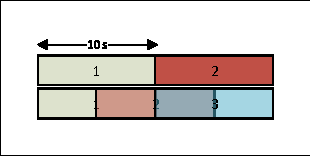
\includegraphics[clip=true, trim=5mm 5mm 5mm 5mm]{img/interval_overlap}
\caption{Intervallüberlappung}
\label{tab:interval-overlap}
\end{table}

Bao et al. nutzten 2004 auf der Basis bereits bestehender Werke für die Transformation eine Intervallüberlappung von $50 \%$ \cite{Bao2004}. Weiss et al. probierten dies laut ihrem Paper nicht aus \cite{Weiss2016}. Um zu prüfen, ob dies eine weitere Verbesserung der Genauigkeiten erzielen könnte, wurden für die Intervalle $(t_0, t_0 + 10), ((t_0 + 10) - 10 * 0.5, (t_0 + 10) - 10 * 0.5 + 10), ...$ Features generiert und wie zuvor evaluiert. Eine Illustration der Überlappung befindet sich in Tabelle~\ref{tab:interval-overlap}.

Anders als erhofft verschlechterten sich die persönlichen RF-Modelle wie in Tabelle~\ref{tab:accuracy-overlap} ersichtlich durch die Überlappung um $0.2 \%$, während sich die unpersönlichen Modelle sogar um $5.1 \%$ verschlechterten.

\begin{table}
\centering
\begin{tabular}{|c|c|c||c|c|}
	\hline 
	\textbf{Algo.} & \textbf{Comb. (Pers.)} & \textbf{Überlappung (Pers.)} &\textbf{Comb. (Unpers.)} & \textbf{Überlappung (Unpers.)} \\ 
	\hline 
	RF & \textbf{99.4} & \textbf{99.2} & \textbf{78.5} & \textbf{73.4} \\ 
	J48 & 92.8 & 96.3 & 59.7 & 57.5 \\ 
	IB3 & 82.3 & 81.8 & 52.9 & 50.7 \\ 
	NB & 96.2 & 95.8 & 60.9 & 59.7 \\ 
	MLP & 94.8 & 95.0 & 54.9 & 59.4 \\ 
	\hline 
	$\varnothing$ & 93.1 & 93.6 & 61.4 & 60.9 \\ 
	\hline
\end{tabular} 
\caption{Genauigkeit der Modelle mit Intervallüberlappung in Prozent}
\label{tab:accuracy-overlap}
\end{table}

\section{Genauigkeit bei Verschmelzung der Ess- und Trinkaktivitäten}
\begin{table}
\centering
\begin{tabular}{|c|c|c|}
	\hline 
	\textbf{Algo.} & \textbf{Comb. (Unpers.), verschmolzen} & \textbf{Comb. (Unpers.), nicht verschmolzen} \\ 
	\hline 
	RF & \textbf{87.1} &  \textbf{78.5} \\ 
	J48 & 73.7 &  59.7 \\ 
	IB3 & 63.9 &  52.9  \\ 
	NB & 72.4 & 60.9  \\ 
	MLP & 77.6  & 54.9 \\ 
	\hline 
	$\varnothing$ & 74.9 & 61.4  \\ 
	\hline
\end{tabular} 
\caption{Genauigkeit der Modelle bei Verschmelzung der Ess- und Trinkaktivitäten in Prozent}
\label{tab:accuracy-merge-eating}
\end{table}
\todo{Confusion-Matrix all impersonal rf einbinden}
Betrachtet man die Konfusionsmatrix der vollständigen unpersönlichen RF-basierten Modelle, so lässt sich feststellen, dass die Klassen, die sich mit Essen oder Trinken beschäftigen, nur ungenau erkannt werden und somit die Durchschnittsgenauigkeit entsprechend senken. Zudem liegt die fehlerhaft vorhergesagte Klasse häufig \todo{Zahl nennen} im Bereich des Essens und Trinkens. Zurückzuführen ist dies auf die Tatsache, dass sich diese Aktivitäten untereinander ähneln, da die zentralen Bewegungsmerkmale das Sitzen sowie das Führen der Hand zum Mund sind.

Tabelle~\ref{tab:accuracy-merge-eating} zeigt, wie sich die Genauigkeit der unpersönlichen Modelle verändert, wenn man diese Aktivitäten zu einer einzigen Aktivität verschmilzt. \todo{Zeige auch neue Konfusionsmatrix.} Bei den RF-Modellen ist eine Verbesserung um $8.6 \%$ zu erkennen, wovon ein Teil auch darauf zurückzuführen sein könnte, dass es insgesamt weniger Klassen gibt und die Wahrscheinlichkeit einer Fehlklassifikation somit sinkt.

Aus diesen Daten lässt sich schließen, dass bei der Verwendung von unpersönlichen Modellen darauf geachtet werden sollte, dass die zu erkennenden Aktivitäten nicht zu feingranular voneinander getrennt werden, da dies die Klassifikation stark erschweren kann.

% vim: set ft=tex
